% B2 (CsCl) cell of CuZn, used by report.tex and slides.tex (needs tikz).
% Oblique projection: x to the right, y into the page, z up.
\definecolor{cu}{HTML}{EB6834}
\definecolor{zn}{HTML}{2A78D6}
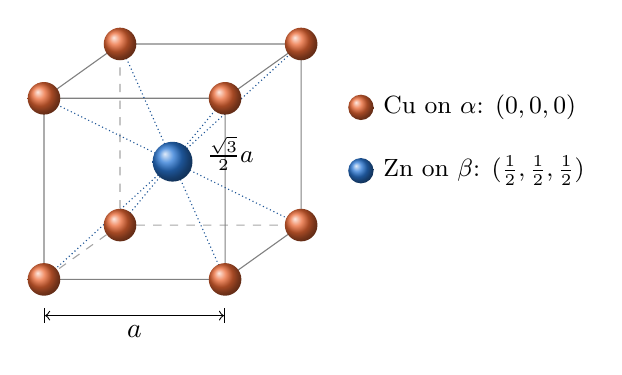
\begin{tikzpicture}[x={(1cm,0cm)}, y={(0.42cm,0.3cm)}, z={(0cm,1cm)}, scale=2.3, line join=round]
  % cube edges: the three edges of the back-bottom-left corner are hidden
  \draw[gray!70, dashed, thin] (0,1,0) -- (0,0,0)  (0,1,0) -- (1,1,0)  (0,1,0) -- (0,1,1);
  \draw[gray, thin] (0,0,0) -- (1,0,0) -- (1,0,1) -- (0,0,1) -- cycle
                    (1,0,0) -- (1,1,0) -- (1,1,1) -- (1,0,1)
                    (0,0,1) -- (0,1,1) -- (1,1,1);
  % the 8 first-neighbour bonds of the centre site
  \foreach \x in {0,1} \foreach \y in {0,1} \foreach \z in {0,1}
    \draw[zn!70!black, densely dotted] (0.5,0.5,0.5) -- (\x,\y,\z);
  % atoms, from the back to the front
  \foreach \x/\z in {0/0,1/0,0/1,1/1} \shade[ball color=cu] (\x,1,\z) circle (0.9mm);
  \shade[ball color=zn] (0.5,0.5,0.5) circle (1.1mm);
  \foreach \x/\z in {0/0,1/0,0/1,1/1} \shade[ball color=cu] (\x,0,\z) circle (0.9mm);
  % distances: a between corners (2nd neighbours), sqrt(3)a/2 corner-centre (1st neighbours)
  \draw[|<->|, thin] (0,0,-0.2) -- (1,0,-0.2) node[midway, below] {$a$};
  \node[font=\small, anchor=west] at (0.74,0.25,0.62) {$\frac{\sqrt{3}}{2}a$};
  % key
  \shade[ball color=cu] (1.75,0,0.95) circle (0.7mm);
  \node[anchor=west, font=\small] at (1.82,0,0.95) {Cu on $\alpha$: $(0,0,0)$};
  \shade[ball color=zn] (1.75,0,0.6) circle (0.7mm);
  \node[anchor=west, font=\small] at (1.82,0,0.6) {Zn on $\beta$: $(\frac12,\frac12,\frac12)$};
\end{tikzpicture}
